%%%%%%%%%%%%%%%%%%%%%%%%%%%%%%%%%%%%%%%%%%%%%%%%%%%%%%%%%%%%%%%%%%%%%
% Henriekes Mitschrieb vom 07.11.2013                               %
%%%%%%%%%%%%%%%%%%%%%%%%%%%%%%%%%%%%%%%%%%%%%%%%%%%%%%%%%%%%%%%%%%%%%
\chapter{Mannigfaltigkeiten und Simpizidkomplexe}
\section{Topologische Mannigfaltigkeiten}
\begin{definition}
    Sei $X$ ein topologischer Raum und $n \in \mdn$.
    \begin{enumerate}[label=(\alph*)]
        \item Eine $n$-dimensionale \textbf{Karte}\xindex{Karte} auf
              $X$ ist ein Paar $(U, \varphi)$, wobei $U \subseteq X$
              offen und $\varphi: U \rightarrow V$ Homöomorphismus
              von $U$ auf eine offene Teilmenge $V \subseteq \mdr^n$.
        \item Ein $n$-dimensionaler \textbf{Atlas}\xindex{Atlas} auf $X$ ist eine
              Familie $(U_i, \varphi_i)_{i \in I}$ von Karten auf $X$,
              sodass $\bigcup_{i \in I} U_i = X$.
        \item $X$ heißt (topologische) $n$-dimensionale \textbf{Mannigfaltigkeit}\xindex{Mannigfaltigkeit},
              wenn $X$ hausdorffsch ist, eine abzählbare Basis der 
              Topologie hat und ein $n$-dimensionalen Atlas besitzt.
    \end{enumerate}
\end{definition}

\begin{bemerkung}
    \begin{enumerate}[label=(\alph*)]
        \item Es gibt surjektive, stetige Abbildungen $[0,1] \rightarrow [0,1] \times [0,1]$
        \item Für $n \neq m$ sind $\mdr^n$ und $\mdr^m$ nicht homöomorph.
              Zum Beweis benutzt man den \enquote{Satz von der Gebietstreue} (Brouwer):

              Ist $U \subseteq \mdr^n$ offen und $f: U \rightarrow \mdr^n$
              stetig und injektiv, so ist $f(U)$ offen.

              Ist $n < m$ und $\mdr^m$ homöomorph zu $\mdr^n$, so wäre
              \[f:\mdr^n \rightarrow \mdr^m \rightarrow \mdr^n, \;\;\; (x_1, \dots, x_n) \mapsto (x_1, x_2, \dots, x_n, 0, \dots, 0)\]
              eine stetige injektive Abbildung. Also müsste $f(\mdr^n)$
              offen sein $\Rightarrow$ Widerspruch
    \end{enumerate}
\end{bemerkung}

\begin{beispiel}
    \begin{enumerate}[label=\arabic*)]
        \item Jede offene Teilmenge $U \subseteq \mdr^n$ ist eine 
              $n$-dimensionale Mannigfaltigkeit mit einem Atlas aus 
              einer Karte.
        \item $\mdc^n$ ist eine $2n$-dimensionale Mannigfaltigkeit
              mit einem Atlas aus einer Karte:
              \[(z_1, \dots, z_n) \mapsto (\operatorname{Re} z_1, \operatorname{Im}z_1, \dots, \operatorname{Re}z_n, \operatorname{Im}z_n)\]
        \item $\mdp^n(\mdr) = (\mdr^{n+1} \setminus \Set{0})/_\sim = S^n /_\sim$ und $\mdp^n(\mdc)$ sind Mannigfaltigkeiten 
              der Dimension $n$ bzw. $2n$.

              $\mdp^n(\mdr) = \bigcup_{i=0}^n U_i,$
              \begin{align*}
U_i = \Set{(x_0: \dots : x_n) \in \mdp^n(\mdr) | x_i \neq 0} &\rightarrow \mdr^n\\
                (x_0 : \dots : x_n) &\mapsto \left (\frac{x_0}{x_i}, \dots, \frac{x_i}{x_i}, \dots, \frac{x_n}{x_i} \right )\\
                (y_1 : \dots : y_{i-1} : 1 : y_i : \dots : y_n) &\mapsfrom (y_1, \dots, y_n)
              \end{align*}
              ist bijektiv.

              Die $U_i,\; i = 0, \dots, n$ bilden einen $n$-dimensionalen Atals.
              \begin{align*}
                      x &= (1:0:0)            &y &= (0:1:1) \in U_2 \rightarrow \mdr^2\\
                \in U_0 &\rightarrow \mdr^2   &y &\mapsto (0,1)\\
                      x &\mapsto (0,0)        &&\text{Umgebung: } \fB_1 (0,1) \rightarrow \Set{(w:z:1) | w^2 + z^2 < 1} = V_2
              \end{align*}
              Umgebung $\fB_1(0,1) \rightarrow \Set{(1:u:v) | \|(u,v)\| < 1} = v_1$

              $V_1 \cap V_2 = \emptyset$?

              $(a:b:c) \in V_1 \cap V_2$\\
              $\Rightarrow a \neq 0$ und $(\frac{b}{a})^2 + (\frac{c}{a})^2 < 1 \Rightarrow \frac{c}{a} < 1$\\
              $\Rightarrow c \neq 0$ und $(\frac{a}{c})^2 + (\frac{b}{c})^2 < 1 \Rightarrow \frac{a}{c} < 1$\\
              $\Rightarrow$ Widerspruch
        \item $S^n = \Set{x \in \mdr^{n+1} | \|x\| = 1}$ ist $n$-dimensionale
              Mannigfaltigkeit.

              Karten: $O_i := \Set{(x_1, \dots, x_{n+1}) \in S^n | x_i > 0} \rightarrow \fB_1 (\underbrace{0, \dots, 0}_{\in \mdr^n})$\\
              $(x_1, \dots, x_{n+1}) \mapsto (x_1, \dots, x_i, \dots, x_{n+1})$\\
              $(x_1, \dots, x_{i-1}, \sqrt{1-\sum_{k=1}^n x_k^2}, x_i, \cdots, x_n)\mapsfrom (x_1, \dots, x_n)$\\
              $S^n = \bigcup_{i=1}^{n+1} (C_i \cup D_i)$
        \item $[0,1]$ ist keine Mannigfaltigkeit, denn:\\
              Es gibt keine Umgebung von $0$ in $[0,1]$, die homöomorph
              zu einem offenem Intervall ist.
        \item $V_1 = \Set{(x,y) \in \mdr^2 | x \cdot y = 0}$ ist
              keine Mannigfaltigkeit.
        \item $V_2 = \Set{(x,y) \in \mdr^2 | x^3 = y^2}$ ist eine
              Mannigfaltigkeit.
        \item $X = (\mdr \setminus \Set{0}) \cup (O_1, O_2)$

              \[U \subseteq X \text{ offen } \gdw 
                \begin{cases}
                    U \text{ offen in } \mdr \setminus \Set{0}, &\text{falls } O_1 \notin U, O_2 \in U\\
                    \exists \varepsilon > 0 \text{ mit } (-\varepsilon, \varepsilon) \subseteq U &\text{falls } O_1 \in U, O_2 \in U
                \end{cases}\]
              Insbesondere sind $(\mdr \setminus \Set{0}) \cup \Set{O_1}$
              und $(\mdr \setminus \Set{0}) \cup \Set{O_2}$ offen und
              homöomorph zu $\mdr$.

              \underline{Aber:} $X$ ist nicht hausdorffsch!
              Denn es gibt keine disjunkten Umgebungen von $O_1$ und
              $O_2$.
        \item $\GL_n(\mdr)$ ist eine Mannigfaltigkeit der Dimension 
              $n^2$, weil offene Teilmengen von $\mdr^{n^2}$ eine
              Mannigfaltigkeit bilden.
    \end{enumerate}
\end{beispiel}

%%%%%%%%%%%%%%%%%%%%%%%%%%%%%%%%%%%%%%%%%%%%%%%%%%%%%%%%%%%%%%%%%%%%%
% Mitschrieb vom 14.11.2013                                         %
%%%%%%%%%%%%%%%%%%%%%%%%%%%%%%%%%%%%%%%%%%%%%%%%%%%%%%%%%%%%%%%%%%%%%
\begin{definition}\xindex{Verklebung}
    Seien $X, Y$ $n$-dimensionale Mannigfaltigkeiten, $U \subseteq X$
    und $V \subseteq Y$ offen, $\Phi: U \rightarrow V$ ein Homöomorphismus
    $Z = (X \dcup Y) /_\sim$ mit der von $u \sim \Phi(u) \forall{u \in U}$
    erzeugten Äquivalenzrelation und der von $\sim$ induzierten 
    Quotiententopologie.

    $Z$ heißt \textbf{Verklebung} von $X$ und $Y$ längs $U$ und $V$.
    $Z$ besitzt einen Atlas aus $n$-dimensionalen Karten.
    Falls $Z$ hausdoffsch ist, ist $Z$ eine $n$-dimensionale 
    Mannigfaltigkeit.
\end{definition}

\todo[inline]{Bilder mit Verklebung einfügen}

\begin{korollar}
    Sind $X, Y$ Mannigfaltigkeiten der Dimension $n$ bzw. $m$, so ist
    $X \times Y$ eine Mannigfaltigkeit der Dimension $n+m$.
\end{korollar}

\begin{beweis}
    Produkte von Karten sind Karten. $\qed$
\end{beweis}

\begin{beispiel}
    Mannigfaltigkeiten mit Dimension 1:
    \begin{enumerate}[label=\arabic*)]
        \item Offene Intervalle, $\mdr$, $(0,1)$ sind alle homöomorph
        \item $S^1$
    \end{enumerate}

    Mannigfaltigkeiten mit Dimension 2:
    \begin{enumerate}[label=\arabic*)]
        \item $\mdr^2$
        \item $S^2$ (0 Henkel)
        \item $T^2$ (1 Henkel)
        \item oder mehr Henkel, wie z.B. der Zweifachtorus in Abb. \ref{fig:double-torus}
    \end{enumerate}

    \begin{figure}
        \centering
        \includegraphics[width=0.2\linewidth, keepaspectratio]{figures/Double-torus-illustration.png}
        \caption{Zweifachtorus}
        \label{fig:double-torus}
    \end{figure}
\end{beispiel}

\begin{korollar}
    Sei $n \in \mdn, F:\mdr^n \rightarrow \mdr$ stetig differenzierbar
    und $X = V(F) := \Set{x \in \mdr^n | F(x) = 0}$ das \enquote{vanishing set}.

    Dann gilt:
    \begin{enumerate}[label=\alph*)]
        \item $X$ ist abgeschlossen in $\mdr^n$
        \item Ist $\text{grad}(F)(X) \neq 0 \forall{x \in X}$, so ist
              $X$ eine Mannigfaltigkeit der Dimension $n-1$.  \label{Mannigfaltigkeitskriterium}
    \end{enumerate}
\end{korollar}

\begin{beweis}
    \begin{enumerate}[label=\alph*),ref=\theplaindefinition.\alph*]
        \item Sei $y \in \mdr^n \setminus V(F)$. Weil $F$ stetig ist,
              gibt es $\delta > 0$, sodass $F(\fB_\delta(y)) \subseteq \fB_\varepsilon(F(y))$
              mit $\varepsilon = \frac{1}{2} \|F(y)\|$. Folgt
              $\fB_\delta(y) \cap V(F) = \emptyset \Rightarrow \mdr^n \setminus V(F)$
              ist offen.
        \item Sei $x \in X$ mit $\text{grad}(F)(x) \neq 0$, also
              \obda $\frac{\partial F}{\partial X_1} (x) \neq 0$,
              $x = (x_1, \dots, x_n)$, $x' := (x_2, \dots, x_n) \in \mdr^{n-1}$.
              Der Satz von der impliziten Funktion liefert nun:
              Es gibt Umgebungen $U$ von $x'$ und differenzierbare
              Funktionen $g: U \rightarrow \mdr$, sodass
              $G: U \rightarrow \mdr^n, \; u \mapsto (g(u), u)$
              eine stetige Abbildung auf eine offene Umgebung $V$ von
              $x$ in $X$ ist.
    \end{enumerate}  
    $\qed$
\end{beweis}

\begin{beispiel}\xindex{Neilsche Parabel}
    \begin{enumerate}[label=\alph*)]
        \item $F: \mdr^3 \rightarrow \mdr,\;\;\; (x, y, z) \mapsto x^2 + y^2 + z^2 - 1$,
              $V(F) = S^2$, $\text{grad}(F) = (2x, 2y, 2z) \xRightarrow{\ref{Mannigfaltigkeitskriterium}} S^n$
              ist $n$-dimensionale Mannigfaltigkeit in $\mdr^{n+1}$
        \item $F: \mdr^2 \rightarrow \mdr, \;\;\; (x,y) \mapsto y^2 - x^3$
            \begin{figure}[ht]
                \centering
                \subfloat[$F(x,y) = y^2 - x^3$]{
                    \input{figures/3d-function-semicubical-parabola.tex}
                    \label{fig:semicubical-parabola-2d}
                }%
                \subfloat[$y^2 - ax^3 = 0$]{
                    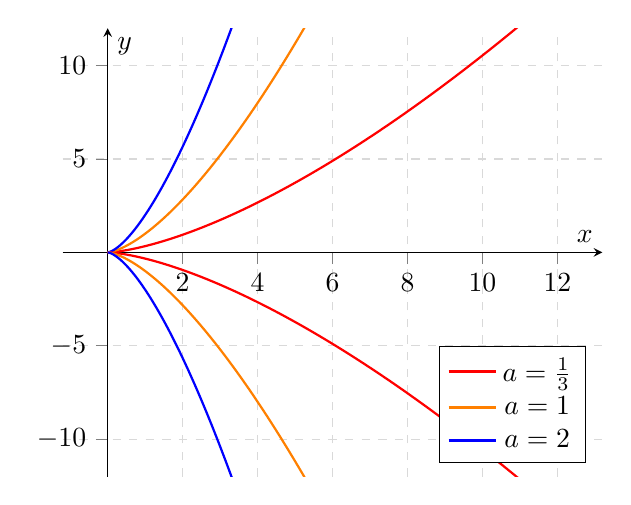
\begin{tikzpicture}
    \begin{axis}[
        legend pos=south east,
        axis x line=middle,
        axis y line=middle,
        grid = major,
        %width=9cm,
        %height=4.5cm,
        grid style={dashed, gray!30},
        xmin= 0,     % start the diagram at this x-coordinate
        xmax= 12,    % end   the diagram at this x-coordinate
        ymin=-10,     % start the diagram at this y-coordinate
        ymax= 10,   % end   the diagram at this y-coordinate
        %axis background/.style={fill=white},
        xlabel=$x$,
        ylabel=$y$,
        %xticklabels={-2,-1.6,...,7},
        tick align=outside,
        %minor tick num=-3,
        enlargelimits=true]
      \addplot[domain=0:12, red, thick,samples=500] {1/3*x^1.5}; 
      \addplot[domain=0:12, orange, thick,samples=500] {1*x^1.5}; 
      \addplot[domain=0:12, blue, thick,samples=500] {2*x^1.5}; 

      \addplot[domain=0:12, red, thick,samples=500] {-1/3*x^1.5}; 
      \addplot[domain=0:12, orange, thick,samples=500] {-1*x^1.5}; 
      \addplot[domain=0:12, blue, thick,samples=500] {-2*x^1.5}; 
      \addlegendentry{$a=\frac{1}{3}$}
      \addlegendentry{$a=1$}
      \addlegendentry{$a=2$}
    \end{axis} 
\end{tikzpicture}

                    \label{fig:semicubical-parabola-3d}
                }%
                \label{Neilsche-Parabel}
                \caption{Rechts ist die Neilsche Parabel für verschiedene Parameter $a$.}
            \end{figure}
              Es gilt: $\text{grad}(F) = (-3x^2, 2y)$. Also: $\text{grad}(0,0) = (0,0)$.
              Daher ist Korollar \label{Mannigfaltigkeitskriterium}
              nicht anwendbar, aber $V(F)$ ist trotzdem
              eine 1-dimensionale topologische Mannigfaltigkeit.
    \end{enumerate}
\end{beispiel}

\begin{definition}\textbf{Mannigfaltigkeit!mit Rand}
    Sei $X$ ein Hausdorffraum mit abzählbarer Basis der Topologie.
    $X$ heißt $n$-dimensionale \textbf{Mannigfaltigkeit mit Rand},
    wenn es einen Atlas $(U_i, \varphi_i)$ gibt, wobei $U_i \subseteq X_i$
    offen und $\varphi_i$ ein Homöomorphismus auf eine offene 
    Teilmenge von 
    \[R_{+,0}^n := \Set{(x_1, \dots, x_n) \in \mdr^n | x_m \geq 0}\]
    ist. $R_{+,0}^n$ ist ein \enquote{Halbraum}.
\end{definition}

\begin{beispiel}
    \todo[inline]{Viele Bilder: Pair of pants, sphere with a hole, halbraum...}
\end{beispiel}

\begin{definition}\xindex{Rand}
    Sei $X$ eine $n$-dimensionale Mannigfaltigkeit mit Rand und
    Atlas $(U_i, \varphi_i)$. Dann heißt 
    \[\partial X := \bigcup_{i\in I} \Set{x \in U_i | \varphi_i (x)_n = 0}\]
    \textbf{Rand} von $X$.
\end{definition}

$\partial X$ ist eine Mannigfaltigkeit der Dimension $n-1$.

\begin{definition}\xindex{Kartenwechsel}\xindex{bergangsfunktion}
    Sei $X$ eine $n$-dimensionale Mannigfaltigkeit mit Atlas
    $(U_i, \varphi_i)_{i \in I}$

    \begin{enumerate}[label=\alph*)]
        \item Für $i, j \in I$ mit $U_i, U_j \neq \emptyset$ heißt
              \begin{align*}
                \varphi_{ij} &:= \varphi_j \circ \varphi_i^{-1}\\
                \varphi_i (U_i \cap U_j) &\rightarrow \varphi_j (U_i \cap U_j)
              \end{align*}
              \textbf{Kartenwechsel} oder \textbf{Übergangsfunktion}.
    \end{enumerate}
\end{definition}

\todo[inline]{Bilder mit Verklebung einfügen}

% Die Übungsaufgaben sollen ganz am Ende des Kapitels sein.
\clearpage
\section*{Übungsaufgaben}
\addcontentsline{toc}{section}{Übungsaufgaben}

\begin{aufgabe}[Zusammenhang]\label{ub4:aufg1}
    \begin{enumerate}[label=(\alph*)]
        \item Beweisen Sie, dass eine topologische Mannigfaltigkeit
              genau dann wegzusammenhängend ist, wenn sie zusammenhängend
              ist
        \item Betrachten Sie nun wie in Beispiel~\ref{bsp:mannigfaltigkeit8}
              den Raum $X:= (\mdr \setminus \Set{0}) \cup \Set{0_1, 0_2}$
              versehen mit der dort definierten Topologie. Ist $X$
              wegzusammenhängend?
    \end{enumerate}
\end{aufgabe}

